% Options for packages loaded elsewhere
\PassOptionsToPackage{unicode}{hyperref}
\PassOptionsToPackage{hyphens}{url}
%
\documentclass[
]{article}
\usepackage{amsmath,amssymb}
\usepackage{iftex}
\ifPDFTeX
  \usepackage[T1]{fontenc}
  \usepackage[utf8]{inputenc}
  \usepackage{textcomp} % provide euro and other symbols
\else % if luatex or xetex
  \usepackage{unicode-math} % this also loads fontspec
  \defaultfontfeatures{Scale=MatchLowercase}
  \defaultfontfeatures[\rmfamily]{Ligatures=TeX,Scale=1}
\fi
\usepackage{lmodern}
\ifPDFTeX\else
  % xetex/luatex font selection
\fi
% Use upquote if available, for straight quotes in verbatim environments
\IfFileExists{upquote.sty}{\usepackage{upquote}}{}
\IfFileExists{microtype.sty}{% use microtype if available
  \usepackage[]{microtype}
  \UseMicrotypeSet[protrusion]{basicmath} % disable protrusion for tt fonts
}{}
\makeatletter
\@ifundefined{KOMAClassName}{% if non-KOMA class
  \IfFileExists{parskip.sty}{%
    \usepackage{parskip}
  }{% else
    \setlength{\parindent}{0pt}
    \setlength{\parskip}{6pt plus 2pt minus 1pt}}
}{% if KOMA class
  \KOMAoptions{parskip=half}}
\makeatother
\usepackage{xcolor}
\usepackage[margin=1in]{geometry}
\usepackage{graphicx}
\makeatletter
\def\maxwidth{\ifdim\Gin@nat@width>\linewidth\linewidth\else\Gin@nat@width\fi}
\def\maxheight{\ifdim\Gin@nat@height>\textheight\textheight\else\Gin@nat@height\fi}
\makeatother
% Scale images if necessary, so that they will not overflow the page
% margins by default, and it is still possible to overwrite the defaults
% using explicit options in \includegraphics[width, height, ...]{}
\setkeys{Gin}{width=\maxwidth,height=\maxheight,keepaspectratio}
% Set default figure placement to htbp
\makeatletter
\def\fps@figure{htbp}
\makeatother
\setlength{\emergencystretch}{3em} % prevent overfull lines
\providecommand{\tightlist}{%
  \setlength{\itemsep}{0pt}\setlength{\parskip}{0pt}}
\setcounter{secnumdepth}{-\maxdimen} % remove section numbering
\ifLuaTeX
  \usepackage{selnolig}  % disable illegal ligatures
\fi
\usepackage{bookmark}
\IfFileExists{xurl.sty}{\usepackage{xurl}}{} % add URL line breaks if available
\urlstyle{same}
\hypersetup{
  pdftitle={Проектирование тонкопленочных гибридных интегральных микросхем},
  hidelinks,
  pdfcreator={LaTeX via pandoc}}

\title{Проектирование тонкопленочных гибридных интегральных микросхем}
\author{}
\date{\vspace{-2.5em}}

\begin{document}
\maketitle

\section{Вариант 29 (1)}\label{ux432ux430ux440ux438ux430ux43dux442-29-1}

\subsection{Исходные
данные}\label{ux438ux441ux445ux43eux434ux43dux44bux435-ux434ux430ux43dux43dux44bux435}

\begin{figure}
\centering
\includegraphics{HW1/Circut2.gif}
\caption{Рисунок 2. Схема чего то}
\end{figure}

Параметры элементов:

\begin{itemize}
\tightlist
\item
  \(R1\): 20 кОм ±10\% 0,01 Вт
\item
  \(R2\): 47 кОм ±20\% 0,02 Вт
\item
  \(R3\): 4.7 кОм ±10\% 0,02 Вт
\item
  \(R4\): 2 кОм ±10\% 0,02 Вт
\item
  \(C1\): 1000 пФ
\item
  \(C2\): 330 пФ
\item
  \(C3\): 1000 пФ
\end{itemize}

\subsection{Расчет параметров
ГИС}\label{ux440ux430ux441ux447ux435ux442-ux43fux430ux440ux430ux43cux435ux442ux440ux43eux432-ux433ux438ux441}

\subsubsection{1. Расчет размеров пленочных
резисторов}\label{ux440ux430ux441ux447ux435ux442-ux440ux430ux437ux43cux435ux440ux43eux432-ux43fux43bux435ux43dux43eux447ux43dux44bux445-ux440ux435ux437ux438ux441ux442ux43eux440ux43eux432}

Опеределим оптимальное удельное поверхностное сопротивление:

\[\rho_□ = \sqrt{\frac{\sum R}{\sum R^{-1}}} = 9695 \text{Ом} \approx 10000 \text{Ом}\]

Материал с ближайшим значением \(\rho_□\), удовлетворяющий необходимому
диапазону значений сопротивления --- \emph{Кермет К-50С} с удельной
мощностью рассеивания \(W_0 = 2\) Вт/см\^{}2.

Определим ширину резисторов \(b_w\), обеспечивающую необходимую мощность
рассеивания:

\[b_w = \sqrt{\frac{\rho_□ \cdot W}{R \cdot W_0}}\]

(Значения округляются в большую сторону до шага сетки \(H = 0.1\) мм)

\[b_{w1}=0.05 \text см \approx 0.6\text{мм},b_{w2}=0.046 \text см \approx 0.5\text{мм},b_{w3}=0.146 \text см \approx 1.5\text{мм},b_{w4}=0.224 \text см \approx 2.3\text{мм}\]

Определим ширину резисторов \(b\) с поправкой на точность изготовления:

\[b_1=0.6\text{мм},b_2=0.5\text{мм},b_3=1.5\text{мм},b_4=2.3\text{мм}\]

Определим длины резисторов:

\[l = \frac{R}{\rho_□}\cdot b = k_ф \cdot b\]

(Значения округляются до ближайшего, кратного шагу сетки \(H = 0.1\) мм)

\[k_{ф1}=2,k_{ф2}=4.7,k_{ф3}=0.47,k_{ф4}=0.2\]\[l_1=1.2\text{мм},l_2=2.35 \approx 2.4\text{мм},l_3=0.705 \approx 0.7\text{мм},l_4=0.46 \approx 0.5\text{мм}\]

Оценим погрешность, вызванную округлением:

\[\Delta R' = \frac{\|R - R'\|}{R}\cdot 100\%,\ R' = \frac{l\cdot\rho_□}{b}\]

\[\Delta R'_1=0\%,\Delta R'_2=2\%,\Delta R'_3=1\%,\Delta R'_4=9\%\]

Для каждого из резисторов погрешность удовлетворяет условию
\(\Delta R' \leq \Delta R\).

\subsubsection{2. Расчет размеров пленочных
конденсаторов}\label{ux440ux430ux441ux447ux435ux442-ux440ux430ux437ux43cux435ux440ux43eux432-ux43fux43bux435ux43dux43eux447ux43dux44bux445-ux43aux43eux43dux434ux435ux43dux441ux430ux442ux43eux440ux43eux432}

Расчет сводится к определению активной площади конденсаторов:

\[S = \frac{C}{C_0}\]

Для минимизации размеров найдем \(C_{min}\), взяв \(S_0 = 0.25\) мм\^{}2
(минимально возможную площадь):

\[C_{min} = min(\frac{C_i}{S_0})\]

\[C_{min_1}=40\text{пФ/см^2 * 10^3},C_{min_2}=12\text{пФ/см^2 * 10^3},C_{min_3}=40\text{пФ/см^2 * 10^3}\]

Наиболее подходящим материалом диэлектрика является \emph{моноокись
германия}, поскольку оно обладает высокой удельной емкостью
\(C_0 = 15 * 10^3\) пФ/см\^{}2.

Рассчитаем площадь конденсаторов с выбранным материалом:

\[S_1=6.66666666666667\text{мм^2},S_2=2\text{мм^2},S_3=6.66666666666667\text{мм^2}\]

\subsubsection{3. Конструирование пленочных межсоединений и контактных
площадок}\label{ux43aux43eux43dux441ux442ux440ux443ux438ux440ux43eux432ux430ux43dux438ux435-ux43fux43bux435ux43dux43eux447ux43dux44bux445-ux43cux435ux436ux441ux43eux435ux434ux438ux43dux435ux43dux438ux439-ux438-ux43aux43eux43dux442ux430ux43aux442ux43dux44bux445-ux43fux43bux43eux449ux430ux434ux43eux43a}

Контактные площадки изготавливаются из алюминия А99.

\subsubsection{4. Проектирование защитного
слоя}\label{ux43fux440ux43eux435ux43aux442ux438ux440ux43eux432ux430ux43dux438ux435-ux437ux430ux449ux438ux442ux43dux43eux433ux43e-ux441ux43bux43eux44f}

Защитный слой может быть изготовлен из любой диэлектрической пленки, за
исключением пятиокиси тантала.

\subsection{Итоговая
схема}\label{ux438ux442ux43eux433ux43eux432ux430ux44f-ux441ux445ux435ux43cux430}

\begin{figure}
\centering
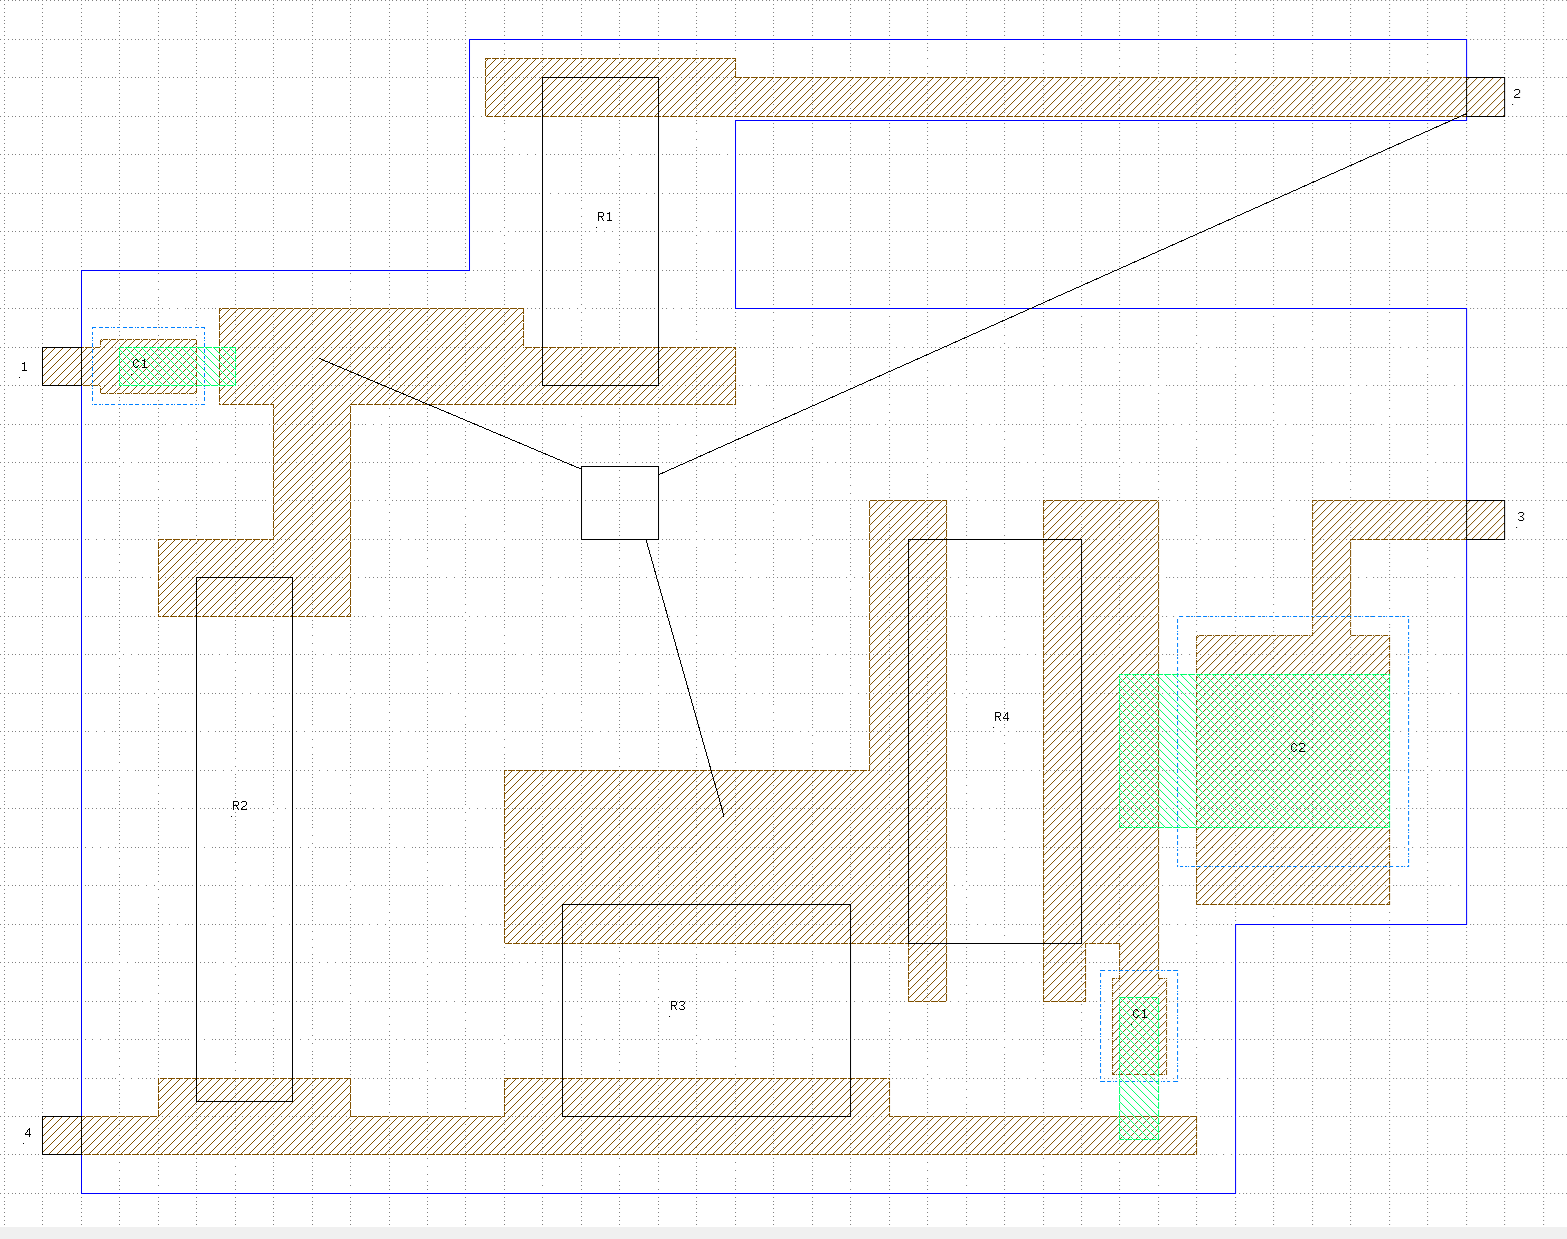
\includegraphics{HW1/myschema.png}
\caption{Рисунок 2. Итоговая схема}
\end{figure}

\end{document}
